\begin{XeClass}{FSOutputSummer}
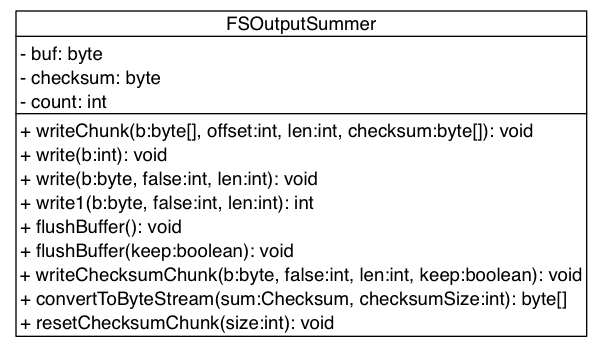
\includegraphics[width=10cm]{cdig/FSOutputSummer.png}
     
 此类是一个抽象类,主要功能是在写入流之前进行校验

    \begin{XeMethod}{\XeProtected \\ \XeAbstract}{void}{writeChunk}
         
 向输出流写入Chunk和其校验和,数据长度为len,位于b字节数组中偏移量为offset的位置。

    \end{XeMethod}

    \begin{XeMethod}{\XePublic \\ \XeSync}{void}{write}
         
 向buffer写入一个字节,在当前buffer满时,flush当前buffer

    \end{XeMethod}

    \begin{XeMethod}{\XePublic \\ \XeSync}{void}{write}
         
 写入数据,数据长度为len,位于b字节数组中偏移量为offset的位置,该方法通过多次
 写入,保证一定会写入len长度的数据,除非发生\emph{IOException}。

    \end{XeMethod}

    \begin{XeMethod}{\XePrivate}{int}{write1}
         
 写入数据,数据长度为len,位于b字节数组中偏移量为offset的位置,如果len大于buf的
 长度,即一个Chunk的大小,那么只写入一个Chunk。
 如果写入的数据小于一个Chunk,那么写入buf,如果len大于buf的剩余容量,则将len
 个字节拷贝到buf中,否则将buf写满,
 如果buf写满,则flush。

    \end{XeMethod}

    \begin{XeMethod}{\XeProtected \\ \XeSync}{void}{flushBuffer}
         
 flush当前的buf,计算并写入checksum,写完后清空buf

    \end{XeMethod}

    \begin{XeMethod}{\XeProtected \\ \XeSync}{void}{flushBuffer}
         
 flush当前的buf,计算并写入checksum,如果keep为true,那么在flush任然保持
 写入之前的状态,即不清空buf。

    \end{XeMethod}

    \begin{XeMethod}{\XePrivate}{void}{writeChecksumChunk}
         
 将buf里的数据Chunk和其对应的校验和写入输出,如果keep为true,则会保持原
 buf的checksum,而不清空。

    \end{XeMethod}

    \begin{XeMethod}{\XePublic}{byte[]}{convertToByteStream}
         
 计算buf中的数据的checksum,返回存放sum的字节数组。

    \end{XeMethod}

    \begin{XeMethod}{\XeProtected \\ \XeSync}{void}{resetChecksumChunk}
         
 重设buf的大小,新的大小为size。

    \end{XeMethod}

\end{XeClass}
